
%%
%% Beuth Hochschule für Technik --  
%%
%% Kapitel 2 - 
%%
%%	

\newpage
[Hansert]
\section{Festlegung des Arbeitpunktes}

Laut Aufgabestellung liegt der Arbeitspunktdruck bei einer Grundlast bei $50Bar$. Da unser System einen Spannungsbereich von 0 bis $10V$ besitzt, müssen wir den Druck in eine Spannung übersetzen.

$Arbeitspunkt = Arbeitspunktdruck * Verstaerkung$\\
$Arbeitspunkt = 50Bar * 0,08V/Bar$\\
$Arbeitspunkt = 4V$\\ 


Um den Arbeitspunkt zu ermitteln muss zuerst das Verhalten des Systems festgestellt werden.


\subsection{Statisches Verhalten}
Um die Kennlinie des Systems zu ermitteln wird, mithilfe des Simulinkmodells \textit{Statische\_Kennlinie.mdl}, eine sprungförmige Erregung mit 20 Schritten, bei jedem Schritt $t= sek$ die Spannung um $0,5V$ erhöht. $t$ wurde so gewählt dass das System einen stationären Zustand erreicht, bevor es neu angeregt wird (Siehe Abbildung \ref{ScopOut} und \ref{ScopIn}).

\begin{figure}[h]
	\begin{center}
		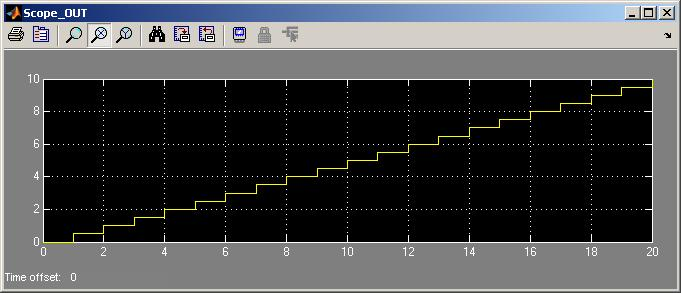
\includegraphics[scale=0.5]{scope_out.jpg}
		\caption{Ausgangssignal, Erregung des Systems}
       \label{ScopOut}
	\end{center} 
\end{figure}


\begin{figure}[h]
	\begin{center}
		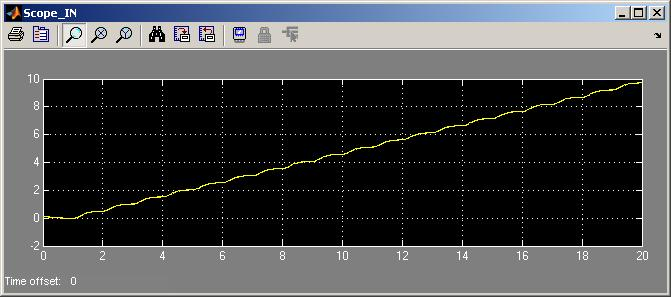
\includegraphics[scale=0.5]{scope_in.jpg}
		\caption{Eingangssignal, Antwort des Systems}
       \label{ScopIn}
	\end{center} 
\end{figure}

Die Antwort wird in der Matrix \textit{ScopeIn.mat} gespeichert und mit dem MATLAB Script \textit{Berechnung\_Kennlinie.m} wird die statische Kennlinie berechnet und gezeichnet (siehe Abbildung \ref{StatKenn}). Um Fehler zu vermeiden haben wir uns dazu entschieden einen Durchschnittswert zu berechnen, dieser besteht aus 20 Werten bevor das System neu erregt wird.


\begin{figure}[h]
	\begin{center}
		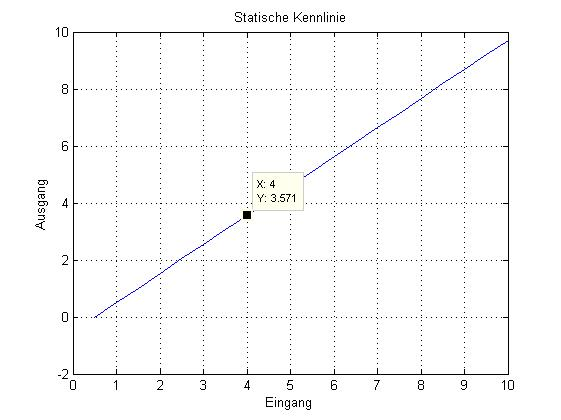
\includegraphics[scale=0.5]{arbeitspunkt.jpg}
		\caption{Statische Kennlinie, Ausgang $y(t)/V$, Eingang $u(t)/V$}
       \label{StatKenn}
	\end{center} 
\end{figure}

In der Abbildung \ref{StatKenn} ist deutlich zu erkennen, dass es sich um eine lineares System handelt, da die Verstärkung konstant bleibt.